\documentclass[11pt]{beamer}
\usetheme{Amsterdam}
\usepackage[utf8]{inputenc}
\usepackage{times}
\usepackage[T1]{fontenc}
\usepackage{tikz}
\usepackage{amsmath}
\usepackage{listings}
\usepackage{adjustbox}

% Default fixed font does not support bold face
\DeclareFixedFont{\ttb}{T1}{txtt}{bx}{n}{12} % for bold
\DeclareFixedFont{\ttm}{T1}{txtt}{m}{n}{12}  % for normal
% Custom colors
\usepackage{color}
\definecolor{deepblue}{rgb}{0,0,0.5}
\definecolor{deepred}{rgb}{0.6,0,0}
\definecolor{deepgreen}{rgb}{0,0.5,0}


% Python style for highlighting
\newcommand\pythonstyle{\lstset{
language=Python,
basicstyle=\ttm,
otherkeywords={self},             % Add keywords here
keywordstyle=\ttb\color{deepblue},
emph={MyClass,__init__},          % Custom highlighting
emphstyle=\ttb\color{deepred},    % Custom highlighting style
stringstyle=\color{deepgreen},
frame=tb,                         % Any extra options here
showstringspaces=false            % 
}}
% Python environment
\lstnewenvironment{python}[1][]
{
\pythonstyle
\lstset{#1}
}
{}

% Python for external files
\newcommand\pythonexternal[2][]{{
\pythonstyle
\lstinputlisting[#1]{#2}}}

% Python for inline
\newcommand\pythoninline[1]{{\pythonstyle\lstinline!#1!}}

\setbeamertemplate{caption}{\insertcaption}
\makeatletter
\def\verbatim{\tiny\@verbatim \frenchspacing\@vobeyspaces \@xverbatim}
\makeatother
% to remove the navigation symbols:
\setbeamertemplate{navigation symbols}{}

%HEAD
\setbeamertemplate{headline}{%
    \begin{beamercolorbox}[colsep=1.3pt]{upper separation line head} \end{beamercolorbox}
    \begin{beamercolorbox}{section in head/foot}
        \vskip2pt\insertsectionnavigationhorizontal{\paperwidth}{}{\hskip0pt plus1filll}\vskip2pt
    \end{beamercolorbox}%
    \begin{beamercolorbox}[ht=12pt]{subsection in head/foot}%
        \vskip2pt\insertsubsectionnavigationhorizontal{\paperwidth}{}{\hskip0pt plus1filll}\vskip2pt
    \end{beamercolorbox}%
    \begin{beamercolorbox}[colsep=1pt]{lower separation line head} \end{beamercolorbox}
}

%FOOT
\setbeamertemplate{footline} {
  \leavevmode%
  \hbox{%
  \begin{beamercolorbox}[wd=.666666\paperwidth,ht=2.25ex,dp=1ex,left]{author in head/foot}%
    \usebeamerfont{author in head/foot} \insertshorttitle \end{beamercolorbox}%
  \begin{beamercolorbox}[wd=.333333\paperwidth,ht=2.25ex,dp=1ex,right]{date in head/foot}%
    \insertframenumber{} / \inserttotalframenumber\hspace*{2ex} \end{beamercolorbox}}%
  \vskip0pt%
}
\setbeamerfont{author}{size=\scriptsize,series=\bfseries,parent=structure}
\setbeamerfont{date}{size=\scriptsize,series=\bfseries,parent=structure}
\title[Aide à la compilation de noyaux Linux]{Aide à la compilation de noyaux Linux}

\subtitle {Projet de programmation}
\author[Aupetit Jordan, Berarde Fabien, Mickaël Lemasson, Bruno Thiao-Layel]
        {Jordan Aupetit \and Fabien Berarde \and Mickaël Lemasson \and Bruno Thiao-Layel}
\date[16 Avril 2014]{
    	    \vspace{-0.5cm}
            \newline Chargé de TD : Xavier Blanc\\
                     Client : Xavier de Rochefort
            \newline
            16 Avril 2014}
\subject{Projet de programmation}

% If you have a file called "university-logo-filename.xxx", where xxx
% is a graphic format that can be processed by latex or pdflatex,
% resp., then you can add a logo as follows:

\pgfdeclareimage[height=0.5cm]{university-logo}{bordeaux-university}
\logo{\pgfuseimage{university-logo}}
\let\reallydohead\dohead
\newenvironment{nonavig}
               {\let\dohead\relax}
               {\let\dohead\reallydohead}

\newlength\someheight
\setlength\someheight{3cm}
\begin{document}

\begin{nonavig}
\begin{frame}
  \titlepage
\end{frame}
\end{nonavig}

\section{Présentation}
\subsection{Objectifs}
\begin{frame}
    \begin{itemize}
        \setlength{\itemsep}{20pt}
        \item Conception d'un outil de configuration de noyaux Linux
        \item Amélioration de certaines fonctionnalités des outils existants
        \item Maintenabilité
        \item Portabilité
    \end{itemize}
\end{frame}

\subsection{Principe}
\begin{frame}
    \begin{figure}
        \includegraphics<1-1>[scale=0.25]{screen_principe_1.png}
        \includegraphics<2-2>[scale=0.25]{screen_principe_2.png}
        \includegraphics<3-3>[scale=0.25]{screen_principe_3.png}
        \includegraphics<4-4>[scale=0.25]{screen_principe_4.png}
        \includegraphics<5-5>[scale=0.25]{screen_principe_5.png}
        \includegraphics<6-6>[scale=0.25]{screen_principe_6.png}
        \centering
    \end{figure}
\end{frame}


\subsection{Kconfig}
\begin{frame}[fragile]
    \begin{figure}
        \caption{Exemple : linux-3.13.5/arch/x86/Kconfig}
        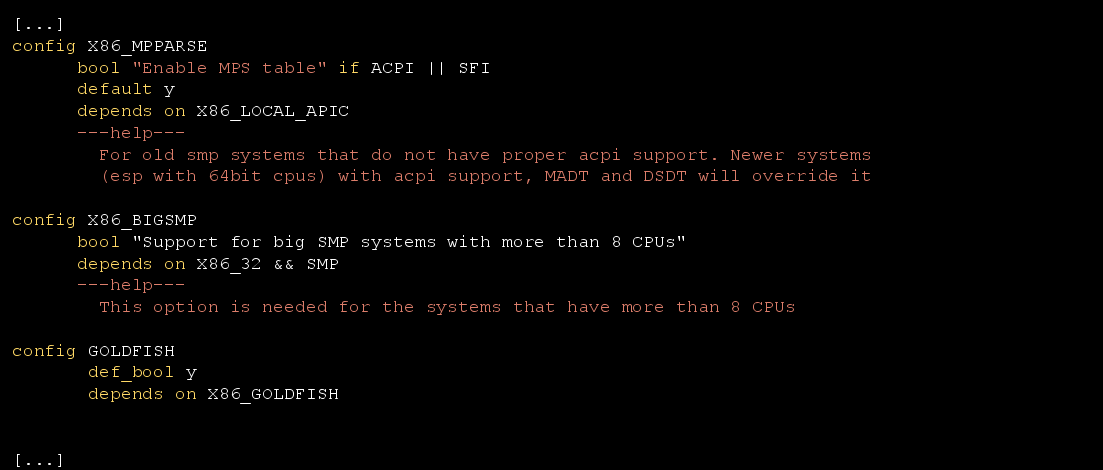
\includegraphics[scale=0.35]{ex_kconfig.png}
        \centering
    \end{figure}
\end{frame}

\subsection{.config}
\begin{frame}[fragile]
    \begin{figure}
        \caption{Exemple : linux-3.13.5/.config}
        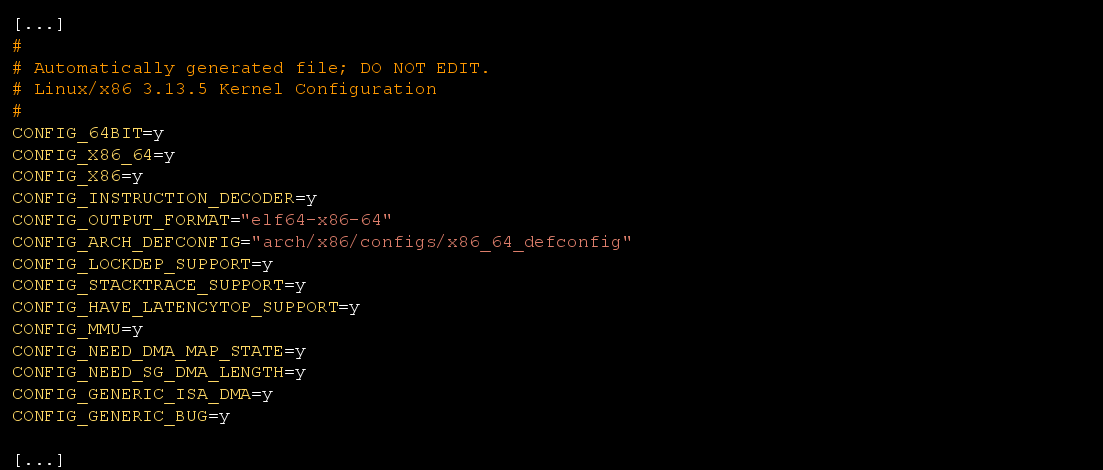
\includegraphics[scale=0.35]{ex_config.png}
        \centering
    \end{figure}
\end{frame}

\section{Existant}
\subsection{Outils existants}
\begin{frame}
    \begin{figure}
        \caption{Exemple en mode console}
        \includegraphics[scale=0.4]<1-1>{conf.png}
        \includegraphics[scale=0.4]<2-2>{mconf.png}
        \centering
    \end{figure}
\end{frame}

\begin{frame}
    \begin{figure}
        \caption{Exemple en mode fenêtré}
        \includegraphics[scale=0.2]<1-1>{gconf.png}
        \includegraphics[scale=0.2]<2-2>{qconf.png}
        \centering
    \end{figure}
\end{frame}
\begin{frame}
    \begin{columns}
    	\begin{column}{6cm}
            \begin{itemize}
                %\setlength{\itemsep}{20pt}
                \item {\color{red} Recherche sur le nom}
                \item Options non modifiables invisibles : conflits
                \item Relation entre les options et le matériel inexistante
            \end{itemize}
    	%\vspace{3cm}
    	\end{column}
    	\begin{column}{4cm}
    		\begin{overprint}
                \begin{tikzpicture}
                    \node[anchor=south west,inner sep=0] (image) at (0,0) {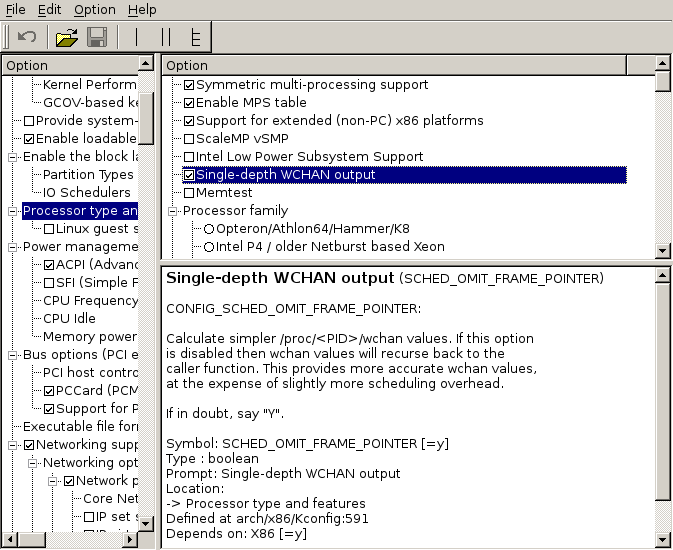
\includegraphics[scale=0.2]{qconf1.png}};
                    \begin{scope}[x={(image.south east)},y={(image.north west)}]
                        \draw[red, thick] (0.59,0.52) rectangle (0.9,0.47);
                        %\draw[help lines,xstep=.1,ystep=.1] (0,0) grid (1,1);
                        %\foreach \x in {0,1,...,9} { \node [anchor=north] at (\x/10,0) {0.\x}; }
                        %\foreach \y in {0,1,...,9} { \node [anchor=east] at (0,\y/10) {0.\y}; }
                    \end{scope}
                \end{tikzpicture}
    		\end{overprint}
    	\end{column}
    \end{columns}
\end{frame}

\subsection{Étude de Waterloo}
\begin{frame}
     \begin{columns}
    	\begin{column}{6cm}
            \begin{itemize}
                \setlength{\itemsep}{20pt}
                \item Kacper Bak et Karim Ali
                \item Redéfinition des besoins
                \item Prototype d'interface
                \begin{itemize}
                    \item Menus
                    \item Progression
                    \item Résoudre les conflits
                \end{itemize}
            \end{itemize}
    	\end{column}

    	\begin{column}{6cm}
    		\begin{overprint}
                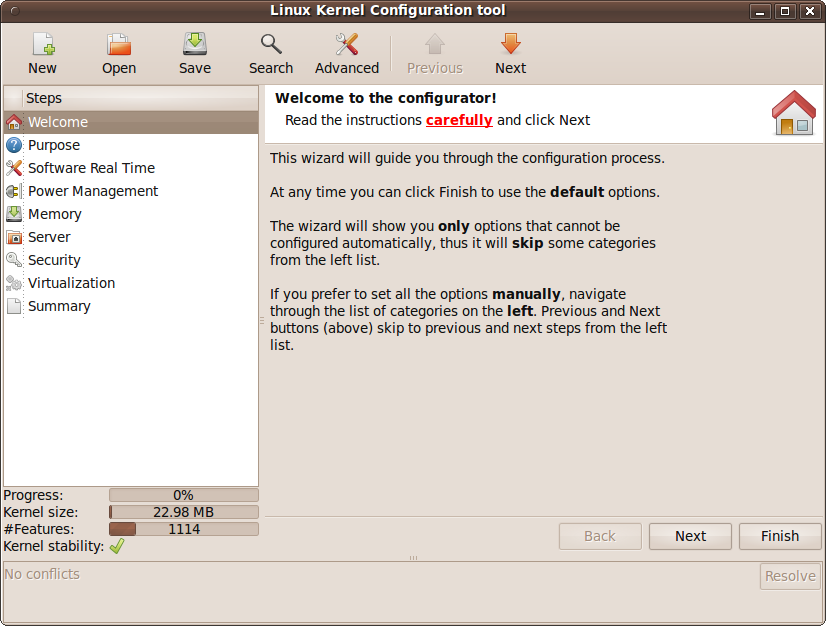
\includegraphics[scale=0.2]{lkc_config.png}
    		\end{overprint}
    	\end{column}
    \end{columns}
\end{frame}

\section{Analyse}
\subsection{Besoins fonctionnels}
\begin{frame}
    \begin{itemize}
        \setlength{\itemsep}{20pt}
        \item Génération et chargement d'un fichier .config
        \item Gestion des conflits
        \item Recherche / filtrage d'option
        \item Détection du matériel
            \begin{itemize}
                \item Correspondance avec des modules Linux
                \item Générer un fichier de configuration minimal
            \end{itemize}
    \end{itemize}
\end{frame}


\subsection{Besoins non fonctionnels}
\begin{frame}
    \begin{itemize}
        \setlength{\itemsep}{20pt}
        \item Portabilité
            \begin{itemize}
                \item Différents système d'exploitation
                \item Interface Web
            \end{itemize}
        \item Architecture modulaire $\rightarrow$ Interface modifiable (Ncurses, QT)
        \item Simplicité / intuitivité $\rightarrow$ Utilisable pour un plus grand large public
    \end{itemize}
\end{frame}


\subsection{Brute-force}
\begin{frame}
    \begin{figure}
        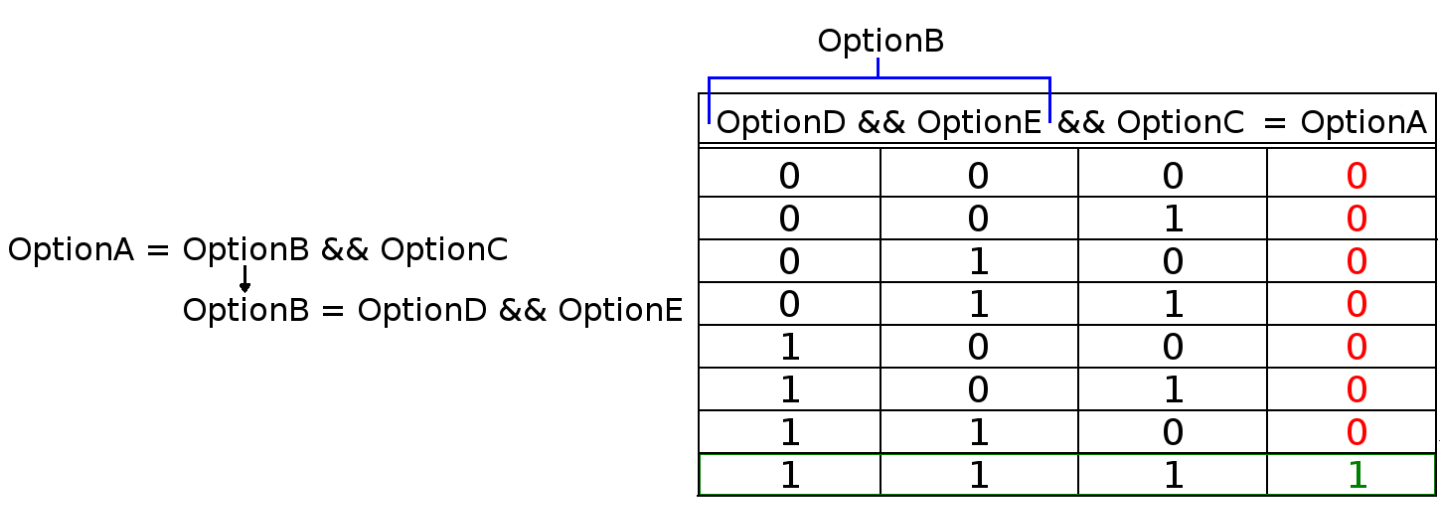
\includegraphics[scale=0.28]{img_diapo_1.png}
        \centering
    \end{figure}
\end{frame}


\subsection{NP-complet}
\begin{frame}
    Soit un ensemble d’options :\\
    \begin{equation}
        (a = true,\; b = true,\; c = false,\; d = false,\; e = true)
    \end{equation}
    et une règle de satisfaisabilité :
    \begin{equation}
        (a \land b \land c) \lor (\lnot c \land d \land e)
    \end{equation}
    La satisfaisabilité est directe.
\end{frame}

\begin{frame}
    Soit un ensemble d’options :\\
    \begin{equation}
    (a = true,\; b = e \;\&\&\; !d,\; c = true,\; d = a,\; e = false)
    \end{equation}
    et la même règle de satisfaisabilité :
    \begin{equation}
        (a \land b \land c) \lor (\lnot c \land d \land e)
    \end{equation}
    On se retrouve à remplacer leurs valeurs :
    \begin{equation}
        (a \land (e \land \lnot d) \land c) \lor (\lnot c \land a \land e)
    \end{equation}
    Difficile de prévoir un état stable.
\end{frame}


\subsection{Get lucky}
\begin{frame}
    \begin{itemize}
        \setlength{\itemsep}{20pt}
        \item Détection des options impliquant un conflit
        \item Tentative de résolution des conflits
        \item Cette résolution de conflit peut aboutir sur un échec
    \end{itemize}
\end{frame}

\begin{frame}
    \begin{figure}
        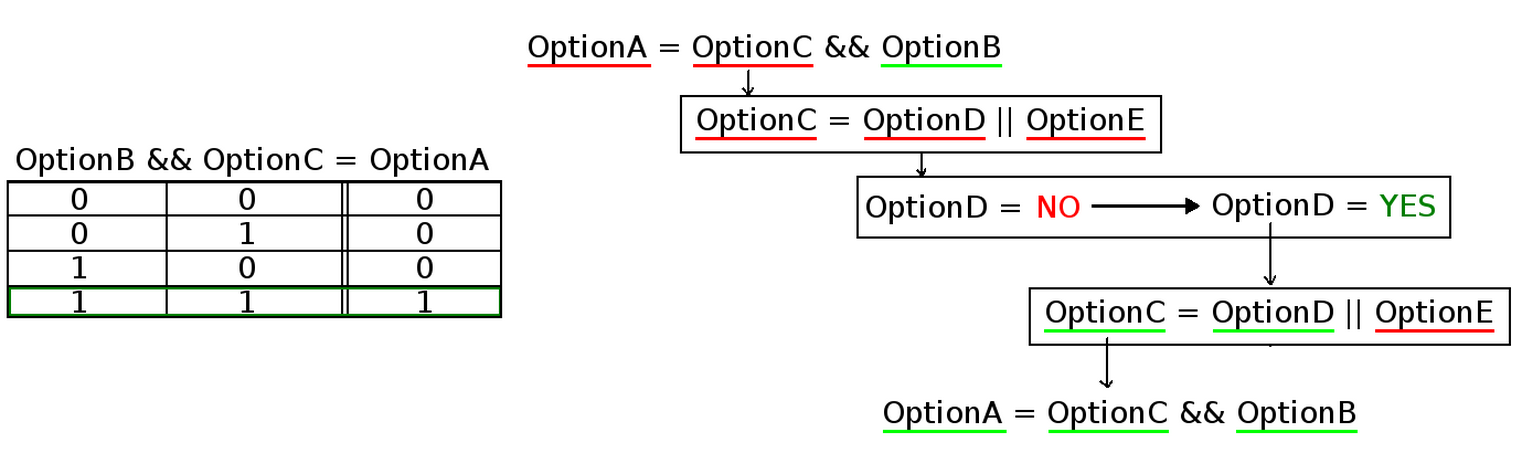
\includegraphics[scale=0.28]{img_diapo_2.png}
        \centering
    \end{figure}
\end{frame}

\section{Développement}
\subsection{Architecture}
\begin{frame}
    \begin{columns}
    	\begin{column}{5cm}
            \begin{itemize}
                \setlength{\itemsep}{20pt}
                \item Langage Python
                \item 3 modules principaux
                    \begin{itemize}
                        \item sync
                        \item core
                        \item render
                    \end{itemize}
                \item Pattern Model View ViewModel
            \end{itemize}
    	\end{column}

    	\begin{column}{6cm}
    		\begin{overprint}
                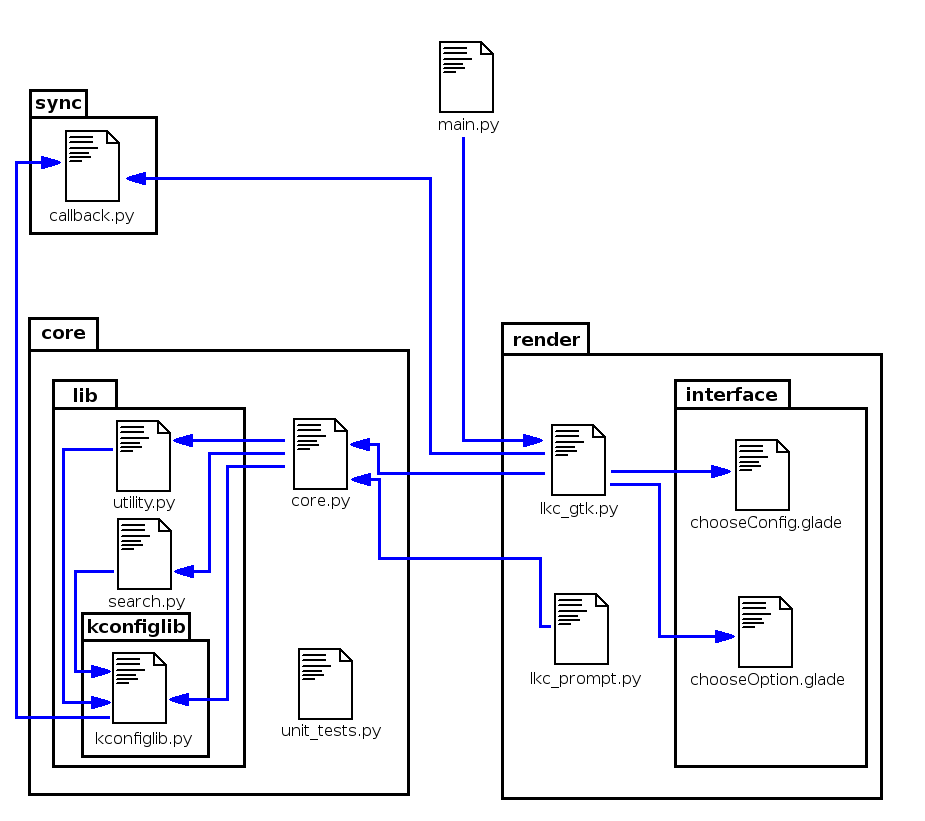
\includegraphics[scale=0.25]{archi_add_v1.png}
    		\end{overprint}
    	\end{column}
    \end{columns}
\end{frame}


\subsection{LKDDb / AutoKernConf}
\begin{frame}
    \begin{itemize}
        \item Génération automatique :
            \begin{itemize}
                \item Liste de correspondance
                \item Fichier de configuration
            \end{itemize}
    	\vspace{0.5cm}
        \item Dernières versions indisponibles (accès via \textit{archive.org})
    	\vspace{0.5cm}
        \item Obsolète
            \begin{itemize}
                \item Incompatible avec les noyaux Linux > 2.6
            \end{itemize}
    \end{itemize}
\end{frame}

\begin{frame}
    \begin{figure}
        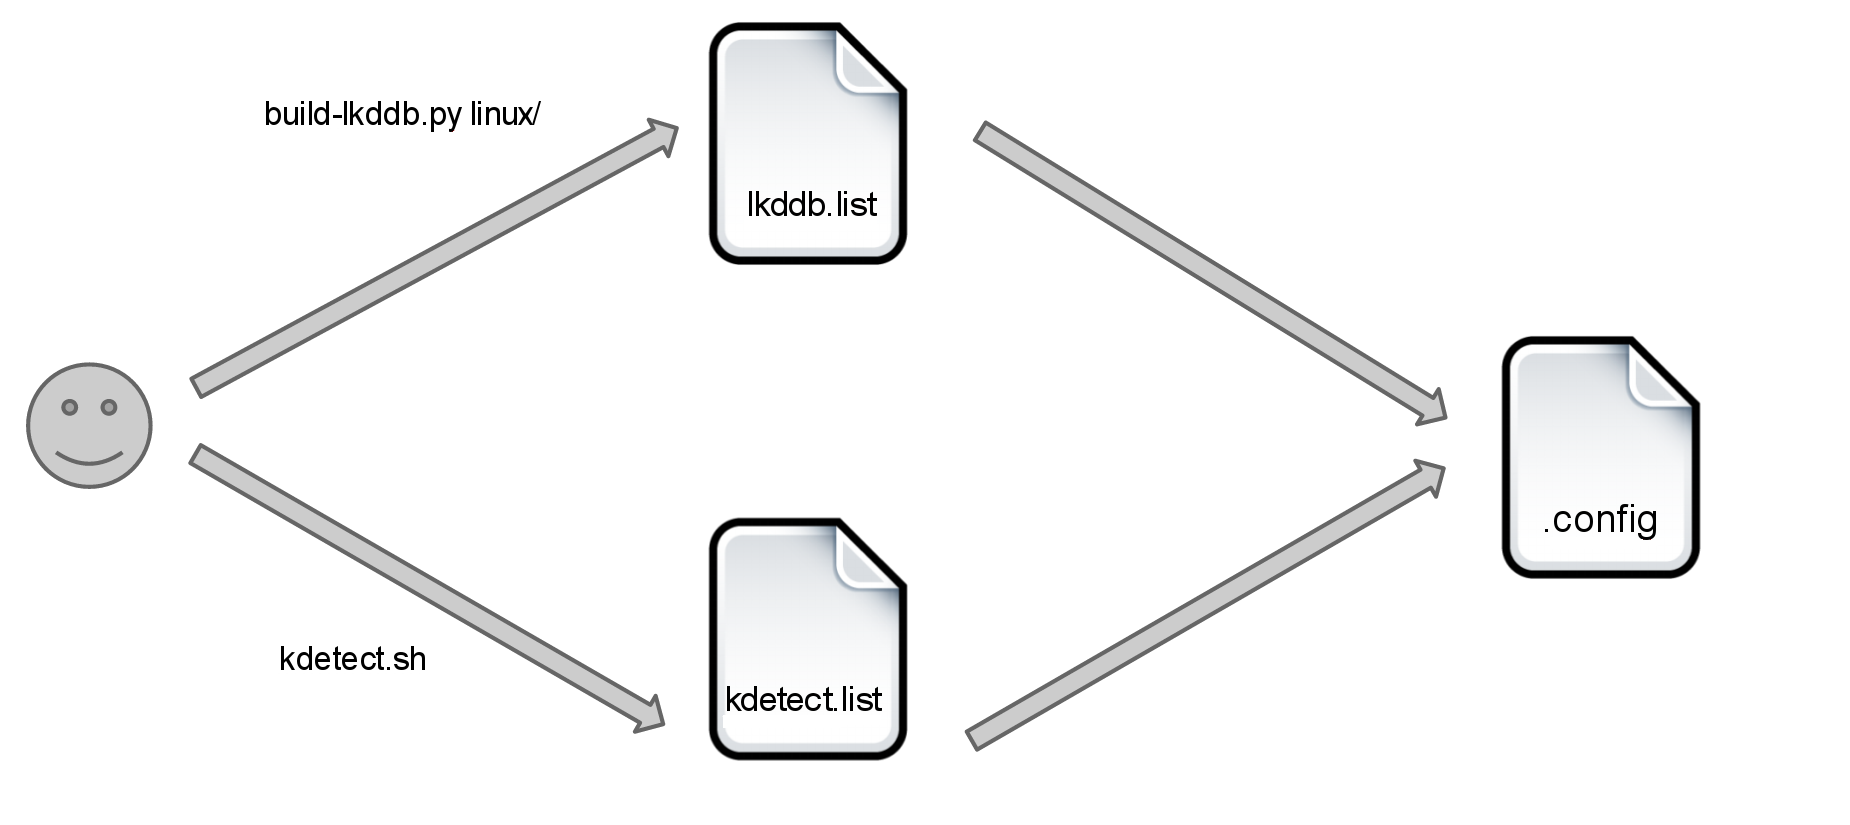
\includegraphics[scale=0.28]{screen_lkddb.png}
        \centering
    \end{figure}
\end{frame}

%MOCHE
\begin{frame}
    \begin{itemize}
        \item Génération automatique :
            \begin{itemize}
                \item Liste de correspondance
                \item Fichier de configuration
            \end{itemize}
    	\vspace{0.5cm}
        \item Dernières versions indisponibles (accès via \textit{archive.org})
    	\vspace{0.5cm}
        \item Obsolète
            \begin{itemize}
                \item Incompatible avec les noyaux Linux > 2.6
            \end{itemize}
    \end{itemize}
\end{frame}
%MOCHE

\subsection{Site communautaire}
\begin{frame}
    \begin{itemize}
        \item Évolution du besoin lié au matériel
    	\vspace{0.5cm}
        \item Une base de données évolutive
    	\vspace{0.5cm}
        \item Une amélioration simple de l'outil
    \end{itemize}
\end{frame}


\subsection{Kconfiglib}
\begin{frame}
    \begin{itemize}
        \item Base du projet
    	\vspace{0.5cm}
        \item Parseur Kconfig en Python
    	\vspace{0.5cm}
        \item Charge / sauvegarde un \textit{.config}
    	\vspace{0.5cm}
        \item Portable
    \end{itemize}
\end{frame}


\subsection{Interface graphique}
\begin{frame}
    \begin{figure}
        \includegraphics<1-1>[scale=0.25]{screen_scenario_1.png}
        \includegraphics<2-2>[scale=0.25]{screen_scenario_2.png}
        \includegraphics<3-3>[scale=0.25]{screen_configuration_interface.png}
        \includegraphics<4-4>[scale=0.25]{screen_scenario_3.png}
        \hspace*{-1cm}\includegraphics<5-5>[scale=0.3]{screen_options_home.png}
        \includegraphics<6-6>[scale=0.4]{screen_search.png}
        \includegraphics<7-7>[scale=0.4]{screen_search_2.png}
        \includegraphics<8-8>[scale=0.4]{screen_search_3.png}
        \includegraphics<9-9>[scale=0.4]{screen_search_4.png}
        \includegraphics<10-10>[scale=0.4]{screen_search_5.png}
        \includegraphics<11-11>[scale=0.4]{screen_search_6.png}
        \includegraphics<12-12>[scale=0.4]{screen_search_7.png}
        \includegraphics<13-13>[scale=0.25]{screen_scenario_4.png}
        \includegraphics<14-14>[scale=0.25]{screen_scenario_5.png}
        \centering
    \end{figure}
\end{frame}


\subsection{Tests}
\begin{frame}[fragile]
    Tests unitaires :
    \begin{itemize}
    	\vspace{0.25cm}
        \item Tests des fonctions de \textit{utility.py}
        \item Exemple : Test de \textit{convert\_xDim\_to\_1Dim}\newline
    \end{itemize}

\begin{adjustbox}{width=\textwidth,height=\someheight,keepaspectratio}
    \begin{python}
test_in = [[[[[[[[["a"]]]]]]]], ["b"], [["c"], ["d"]], [[[["e"]]]]]
test_out = ["a", "b", "c", "d", "e"]
test_res = utility.convert_list_xDim_to_1Dim(test_in)

self.assertEqual(test_res, test_out)

test_in = [[], ["b"], [["c"]], [[[["e"]]]]]
test_out = ["b", "c", "e"]
test_res = utility.convert_list_xDim_to_1Dim(test_in)

self.assertEqual(test_res, test_out)
    \end{python}
\end{adjustbox}
\end{frame}

\begin{frame}
    Tests fonctionnels :
    \begin{itemize}
    	\vspace{0.5cm}
        \setlength{\itemsep}{20pt}
        \item Défilement de toutes les options d'une architecture
        \item Comparaison de la recherche LKC vs outils existants
    \end{itemize}
\end{frame}

\begin{frame}
    Tests non fonctionnels :
    \begin{itemize}
    	\vspace{0.5cm}
        \setlength{\itemsep}{20pt}
        \item Mesure de la vitesse de chargement de l'application
        \item Vérification des fuites de mémoire avec \textit{SMEM}
    \end{itemize}
\end{frame}


\section{Conclusion}
\subsection{Évolutions}
\begin{frame}
    Extensions et améliorations à prévoir :
    \begin{itemize}
    	\vspace{0.5cm}
        \setlength{\itemsep}{20pt}
        \item Lier le site communautaire au logiciel
        \item Ajouter une interface console
        \item Implémenter un système de \textit{get lucky}
        \item Ajouter un système d'annulation de modification
    \end{itemize}
\end{frame}

\subsection{Remerciements}
\begin{frame}
    Nous remercions :
    \begin{itemize}
    	\vspace{0.5cm}
        \setlength{\itemsep}{20pt}
        \item Xavier Blanc
        \item Xavier de Rochefort
        \item Le jury
        \item Kacper Bak et Karim Ali
    \end{itemize}
\end{frame}

\begin{nonavig}
\begin{frame}
    \begin{center}
        {\fontsize{70}{60}\selectfont ?}
    \end{center}
\end{frame}
\end{nonavig}

\end{document}
